\section{Automatic Mode Switching Prediction}
% \section{Training Data}
% In order to train a classifier to recognize the current operation performed by users, we need to collect some usage data as ground truth.
After co-locating the touch sensing and typing device, automatically switching between the touching and typing modes becomes an important issue. We classified the calculated MHIs with Random Decision Forests(RDF) into \emph{keyboard mode} and \emph{trackpad mode} to recognize which mode the user intends to use.
%Final: reviewer 10th request
%In our classifier, the whole frame is classified as "user wants to use trackpad" or "user wants to type", so the system switches between two modes if users' intention changed. 
\subsection{Task Design for collecting training data}
We designed the tasks to meet the following criteria: 1) The tasks must be using both keyboard and touchpad alternately. Switching between two devices occurs frequently. 2) The task was extracted from the regular use of the keyboard and touchpad, and must be simple enough for the users to perform while they also need to operate an extra foot pedal to record their actual intention (see Figure~\ref{fig:pedal}.A). 3) The individual usage times of the keyboard and the touchpad should be as close as possible to each other. This would result in a more balanced dataset, which is better for building a classifier.
\begin{figure}[!b]
\centering
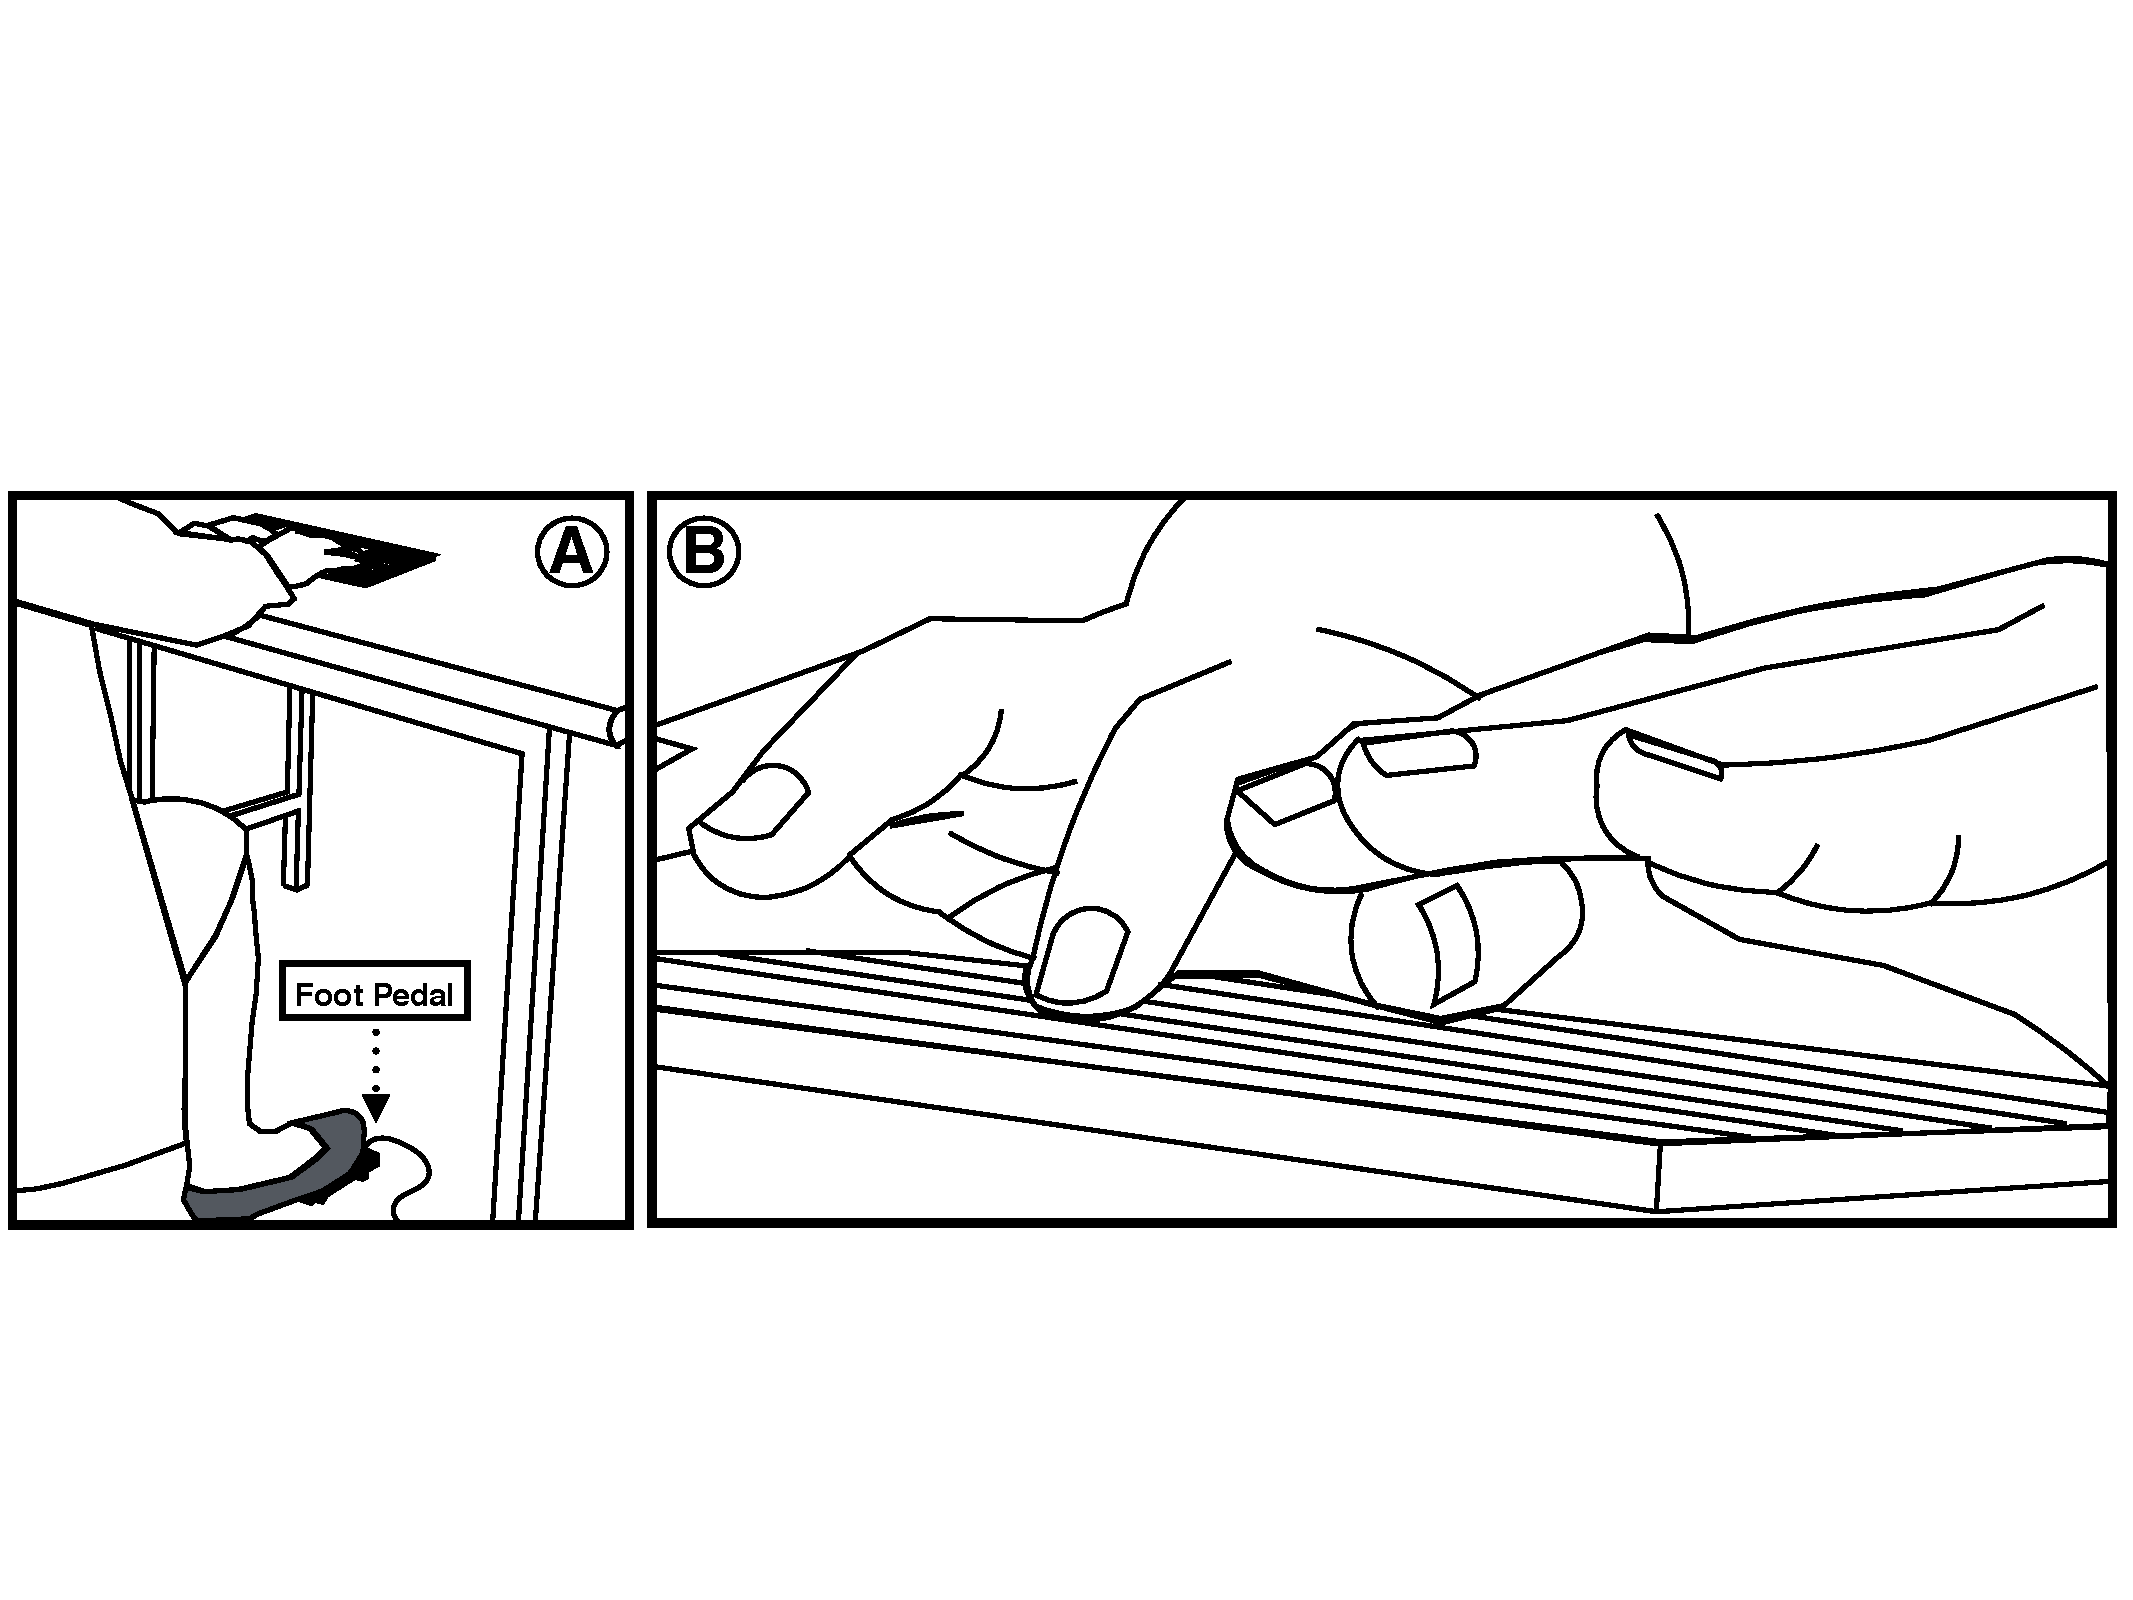
\includegraphics[width=1\columnwidth]{figures/MERGE.pdf}
\caption{(A) Participants switched between typing and pointing by operating the foot pedal manually during the procedure of ground truth collection. Meanwhile, the system labeled each frame according to the current foot pedal's state. (B) A majority of the participants raised their left hand and used one finger of the right hand to perform cursor movements in the trackpad mode.}
\label{fig:pedal}
\end{figure}
\subsection{Procedure}
We recruited 30 participants (15 females, 15 males, mean age 21) with an on-line form.
All participants are right-handed.
In the training session, participants were asked to fill in a questionnaire and learned how to use the foot pedal to switch modes.
In the testing session, participants were asked to use \papertitle\hspace{2pt} to perform the following tasks: 
1) Type a specified sentence in the text processing software.
2) Change the font size of the sentence by moving the mouse cursor to select a different size on the menu bar.
3) Continue typing another sentence and their own name.
4) Insert a picture in the document with the menu button, and resize the picture with the cursor.
5) Close the text processing software and open a web browser.
6) Type "www.facebook.com" in the location bar.
7) Browse the social network site, comment on one of the posts in the news feed.
8) Scroll back to the top of the page and upload a photo.
9) Add some comment on the uploaded photo. Participants were not allowed to use hot keys. They can only type and control the cursor or use a scrolling gesture(two finger swipe).
%The tasks we asked the participants to perform included document editing and typesetting in a text processing software, and browsing a social network site.

All of these tasks were very common tasks for a modern PC user, and should be performed without any difficulties.
Videos of the hand postures and its interaction with the keyboard were recorded for further analysis.
The total operating time of the recorded data is 187.36 minutes, average operating time is 6.24 minutes per user.

\subsection{Labeling}
The ground truth of whether the user is trying to use the keyboard or touchpad is collected with a foot pedal (see Figure~\ref{fig:pedal}.A) switch operated by the participant during the data collection session. Pedal down means pointing and pedal up means typing.
We collected 150007 frames from the training data collection session, 25739 were \emph{keyboard frames}, 61896 were \emph{touchpad frames}.
The remaining 62372 frames were frames without any touched blobs, we call them \emph{blank frames}.
Since those frames didn't contain any touched blobs. We could safely assume that no user operation was being executed at that moment, so we could classify it into neither keyboard nor touchpad frames.
The blank frames were removed from training data while building a classifier, and directly skipped while running on a real-time interactive system, so there would not be any output from our system.

\subsection{Classification Method}
We also implemented Motion Signature \cite{96bytes} to recognize whether the user is trying to use the pointing device or not.
% Since the sample rate is relatively lower (13Hz) compared to the original condition(325Hz), we reduced the referenced frames to only 30 frames in the process of building motion history images(MHI).
Since our sensor's sampling rate of 13Hz is much lower than the sensor used in \cite{96bytes}(325Hz), we only used 30 frames of raw signal to build MHIs. 
Also, we removed binary-MHI(bMHI) from the original MHI implementation because intensity-MHI already provides enough accuracy for recognizing user intention.
We classify the calculated MHIs with Random Decision Forests(RDF), the same classifier used in Type–Hover–Swipe \cite{96bytes}.
%reviewer 9th request
With our hardware system, we can extract touch areas from the image collected with the capacitive sensor grid. Therefore, our system can recognize where the moving touch point is even if the second hand rests on the keyboard. 
% This foot pedal switch also act as a manual mode switch in the system during the data collection session.
%Final: 加圖說明foot pedal用來label training data

\vfill
\columnbreak
%reviewer要求改section name
%\section{Feature Extraction}



